\section{ПРОГРАММЫ И БИБЛИОТЕКИ ДЛЯ МОДЕЛИРОВАНИЯ ТЕЧЕНИЙ}

Численное моделирование течений реактивных струй с неравновесной химией требует применения специализированного программного обеспечения, способного учитывать как газодинамические, так и химико-кинетические процессы. В настоящее время существует ряд коммерческих и открытых пакетов, решающих подобные задачи с различной степенью точности и эффективности. В данном разделе проводится анализ наиболее распространённых программ, рассматриваются их преимущества и ограничения.

\subsection{Коммерческие CFD-пакеты}

\textit{ANSYS Fluent}

Один из самых популярных коммерческих CFD-пакетов, предоставляющий широкие возможности для моделирования турбулентных и химически реагирующих течений.

Плюсы:
\begin{itemize}
    \item поддержка различных моделей турбулентности (RANS, LES, DES);
    \item встроенные базы данных химических реакций и механизмов горения;
    \item удобный графический интерфейс и интеграция с системами CAD/CAE;
    \item чорошая документация и техническая поддержка.
\end{itemize}

Минусы:
\begin{itemize}
    \item платная лицензия;
    \item ограниченная гибкость в настройке пользовательских химических моделей;
    \item значительные вычислительные затраты при расчёте сложных кинетических схем.
\end{itemize}

\textit{COMSOL Multiphysics}

Универсальная платформа для многодисциплинарного моделирования, включая химически реагирующие течения.

Плюсы:
\begin{itemize}
    \item возможность совмещения гидродинамики с другими физическими процессами (теплопередача, электродинамика);
    \item гибкость в задании пользовательских уравнений и граничных условий;
    \item визуализация результатов в реальном времени.
\end{itemize}

Минусы:
\begin{itemize}
    \item менее оптимизирован для высокоскоростных течений по сравнению с узкоспециализированными CFD-пакетами;
    \item ограниченные возможности для моделирования сложной турбулентности;
    \item требует больших ресурсов при расчёте 3D-моделей.
\end{itemize}

\textit{STAR-CCM+}

Мощный CFD-инструмент, разработанный Siemens, с акцентом на промышленные приложения.

Плюсы:
\begin{itemize}
    \item эффективные алгоритмы для расчёта турбулентных и химически реагирующих потоков;
    \item автоматизированное построение сеток и адаптация расчётной области;
    \item поддержка высокопроизводительных вычислений (HPC).
\end{itemize}

Минусы:
\begin{itemize}
    \item сложность освоения для новых пользователей;
    \item высокие требования к вычислительным ресурсам;
    \item ограниченные возможности кастомизации химических моделей.
\end{itemize}

\subsection{Открытые и научно-ориентированные программы} 

\textit{OpenFOAM}

Открытая CFD-платформа, широко используемая в научных исследованиях.

Плюсы:
\begin{itemize}
    \item полная свобода модификации кода и реализации пользовательских моделей;
    \item большое количество готовых решателей для химически реагирующих течений;
    \item бесплатность и поддержка сообщества.
\end{itemize}

Минусы:
\begin{itemize}
    \item сложность настройки и отсутствие удобного графического интерфейса;
    \item требует глубоких знаний численных методов и программирования;
    \item менее оптимизирован для промышленных расчётов по сравнению с коммерческими аналогами.
\end{itemize}

\textit{Cantera}

Библиотека для расчёта химической кинетики и термодинамики, часто используемая совместно с CFD-кодами.

Плюсы:
\begin{itemize}
    \item широкий набор готовых механизмов химических реакций;
    \item интеграция с Python и другими языками программирования;
    \item эффективные алгоритмы расчёта равновесных и неравновесных процессов.
\end{itemize}

Минусы:
\begin{itemize}
    \item не включает полноценные инструменты для гидродинамического моделирования;
    \item требует дополнительной разработки для сопряжения с CFD-решателями.
\end{itemize}

\textit{SU2}

Открытый пакет для моделирования многодисциплинарных задач, включая аэродинамику и горение.

Плюсы:
\begin{itemize}
    \item оптимизирован для задач аэрокосмической тематики;
    \item поддержка адаптивных сеток и параллельных вычислений;
    \item активное развитие и открытый исходный код.
\end{itemize}

Минусы:
\begin{itemize}
    \item ограниченные возможности для моделирования сложной химической кинетики;
    \item меньшее количество документации по сравнению с коммерческими аналогами.
\end{itemize}

\subsection{Сравнительный анализ}

В таблице \ref{tab:tab_compare} представлен сравнительный анализ перечисленных программ по основным критериям.

\begin{table}
    \caption{Таблица сравнения ПО}
    \resizebox{\textwidth}{!} {%
    \begin{tabular}{|c|c|c|c|c|c|}
    \hline
    Критерий & ANSYS Fluent & COMSOL & OpenFOAM & Cantera & SU2 \\
    \hline
    Точность расчётов & Высокая & Средняя & Высокая & Высокая & Высокая \\
    \hline
    Гибкость & Средняя & Высокая & Очень высокая & Очень высокая & Средняя \\
    \hline
    Производительность & Высокая & Средняя & Средняя & Высокая & Высокая \\
    \hline
    Стоимость & Платно & Платно & Бесплатно & Бесплатно & Бесплатно \\
    \hline
    Химические модели  & Широкие & Умеренные & Широкие & Очень широкие & Умеренные \\
    \hline
    \end{tabular}
    }
    \label{tab:tab_compare}
\end{table}

\subsection{Отдельные программы для решения ОДУ и СДУ}

Моделирование неравновесного химического процесса можно представить в виде решения СДУ с начальными условиями. Саму задачу по моделированию течения можно, соответственно, разделить на 2 подзадачи: для течения и для горения. Таким образом, можно использовать одну из программ из предыдущего подраздела отдельно для течений и какую-либо из следующих для решения СДУ химической кинетики. Такой подход может дать более точное решение, хоть и принуждает пользователя использовать сразу несколько ПО и реализовать какие-либо "переходники" между ними.

Программ для решения ОДУ достаточно много~\cite{Wikipedia6, Wikipedia7, Wikipedia8, Wikipedia9, Wikipedia10}. На рисунке \ref{fig:programs} приведены некоторые популярные программы и библиотеки для решения ДУ.

\begin{figure}
    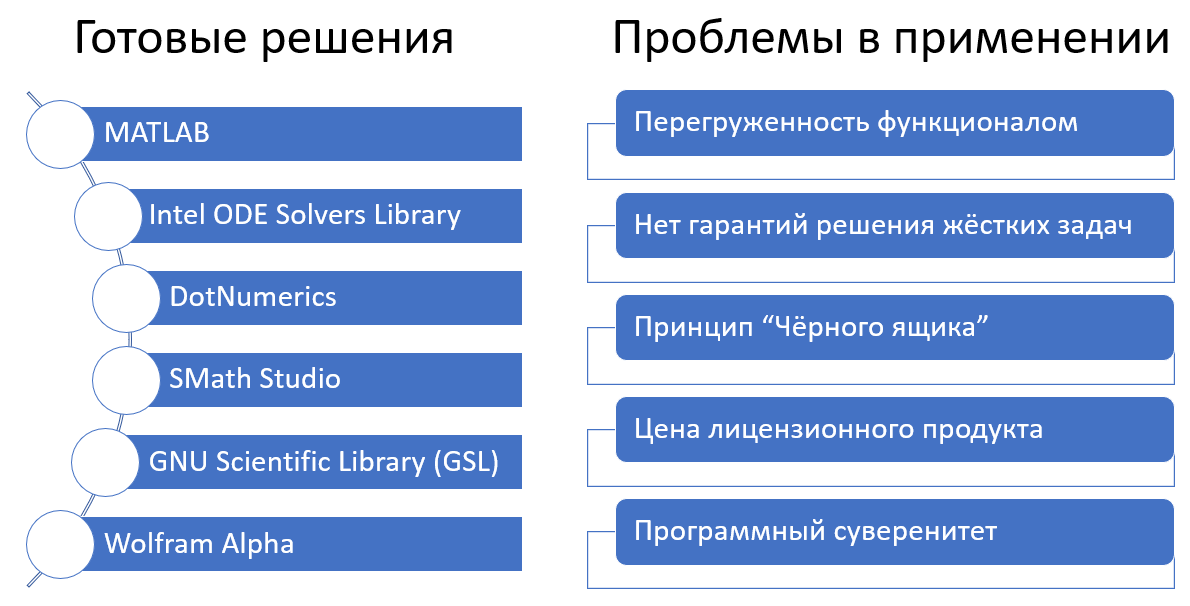
\includegraphics[width=15cm]{2-01-programs}
    \caption{Программы и библиотеки}
    \label{fig:programs}
\end{figure}

Преимущества раздельного подхода:

\begin{itemize}
    \item специализация программного обеспечения,
    \item гибкость выбора моделей,
    \item возможность распределить вычисления на разные потоки.
\end{itemize}

Основные технические сложности:

\begin{itemize}
    \item согласование данных требует разработки интерфейсов,
    \item проблемы устойчивости.
\end{itemize}

\subsection{Общие выводы}

Для промышленных расчётов с жёсткими требованиями к точности и поддержке целесообразно использовать \textit{ANSYS Fluent} или \textit{STAR-CCM+}. В научных исследованиях, где важна гибкость и кастомизация, предпочтительнее \textit{OpenFOAM} в сочетании с \textit{Cantera}. \textit{SU2} подходит для задач, где основное внимание уделено аэродинамике, а химия играет второстепенную роль.

В данной работе в качестве основы была выбрана реализация собственного решателя из-за его открытости, гибкости и возможности интеграции с пользовательскими моделями химической кинетики. Это позволяет реализовать расчёт неравновесных процессов с высокой степенью контроля над алгоритмами.
